\section{Military field}

% Example of applications in the military field
% - Anti jamming and spoofing
% - UAVs
% - Missiles
% - Communication systems

\begin{frame}{IED (Improvised Explosive Devices) Jammers}

    \begin{columns}[c, onlytextwidth]

        \begin{column}{0.5\textwidth}

            IED Jammers are devices that prevent the detonation of IEDs by blocking the radio signals used to trigger them.

            \vspace{10pt}

            A single jammer can cover a limited area, so multiple jammers are used to cover a larger area.
            In order to work together, \textbf{the network must be tightly synchronized}.

        \end{column}

        \hfill

        \begin{column}{0.45\textwidth}

            \begin{figure}
                \centering
                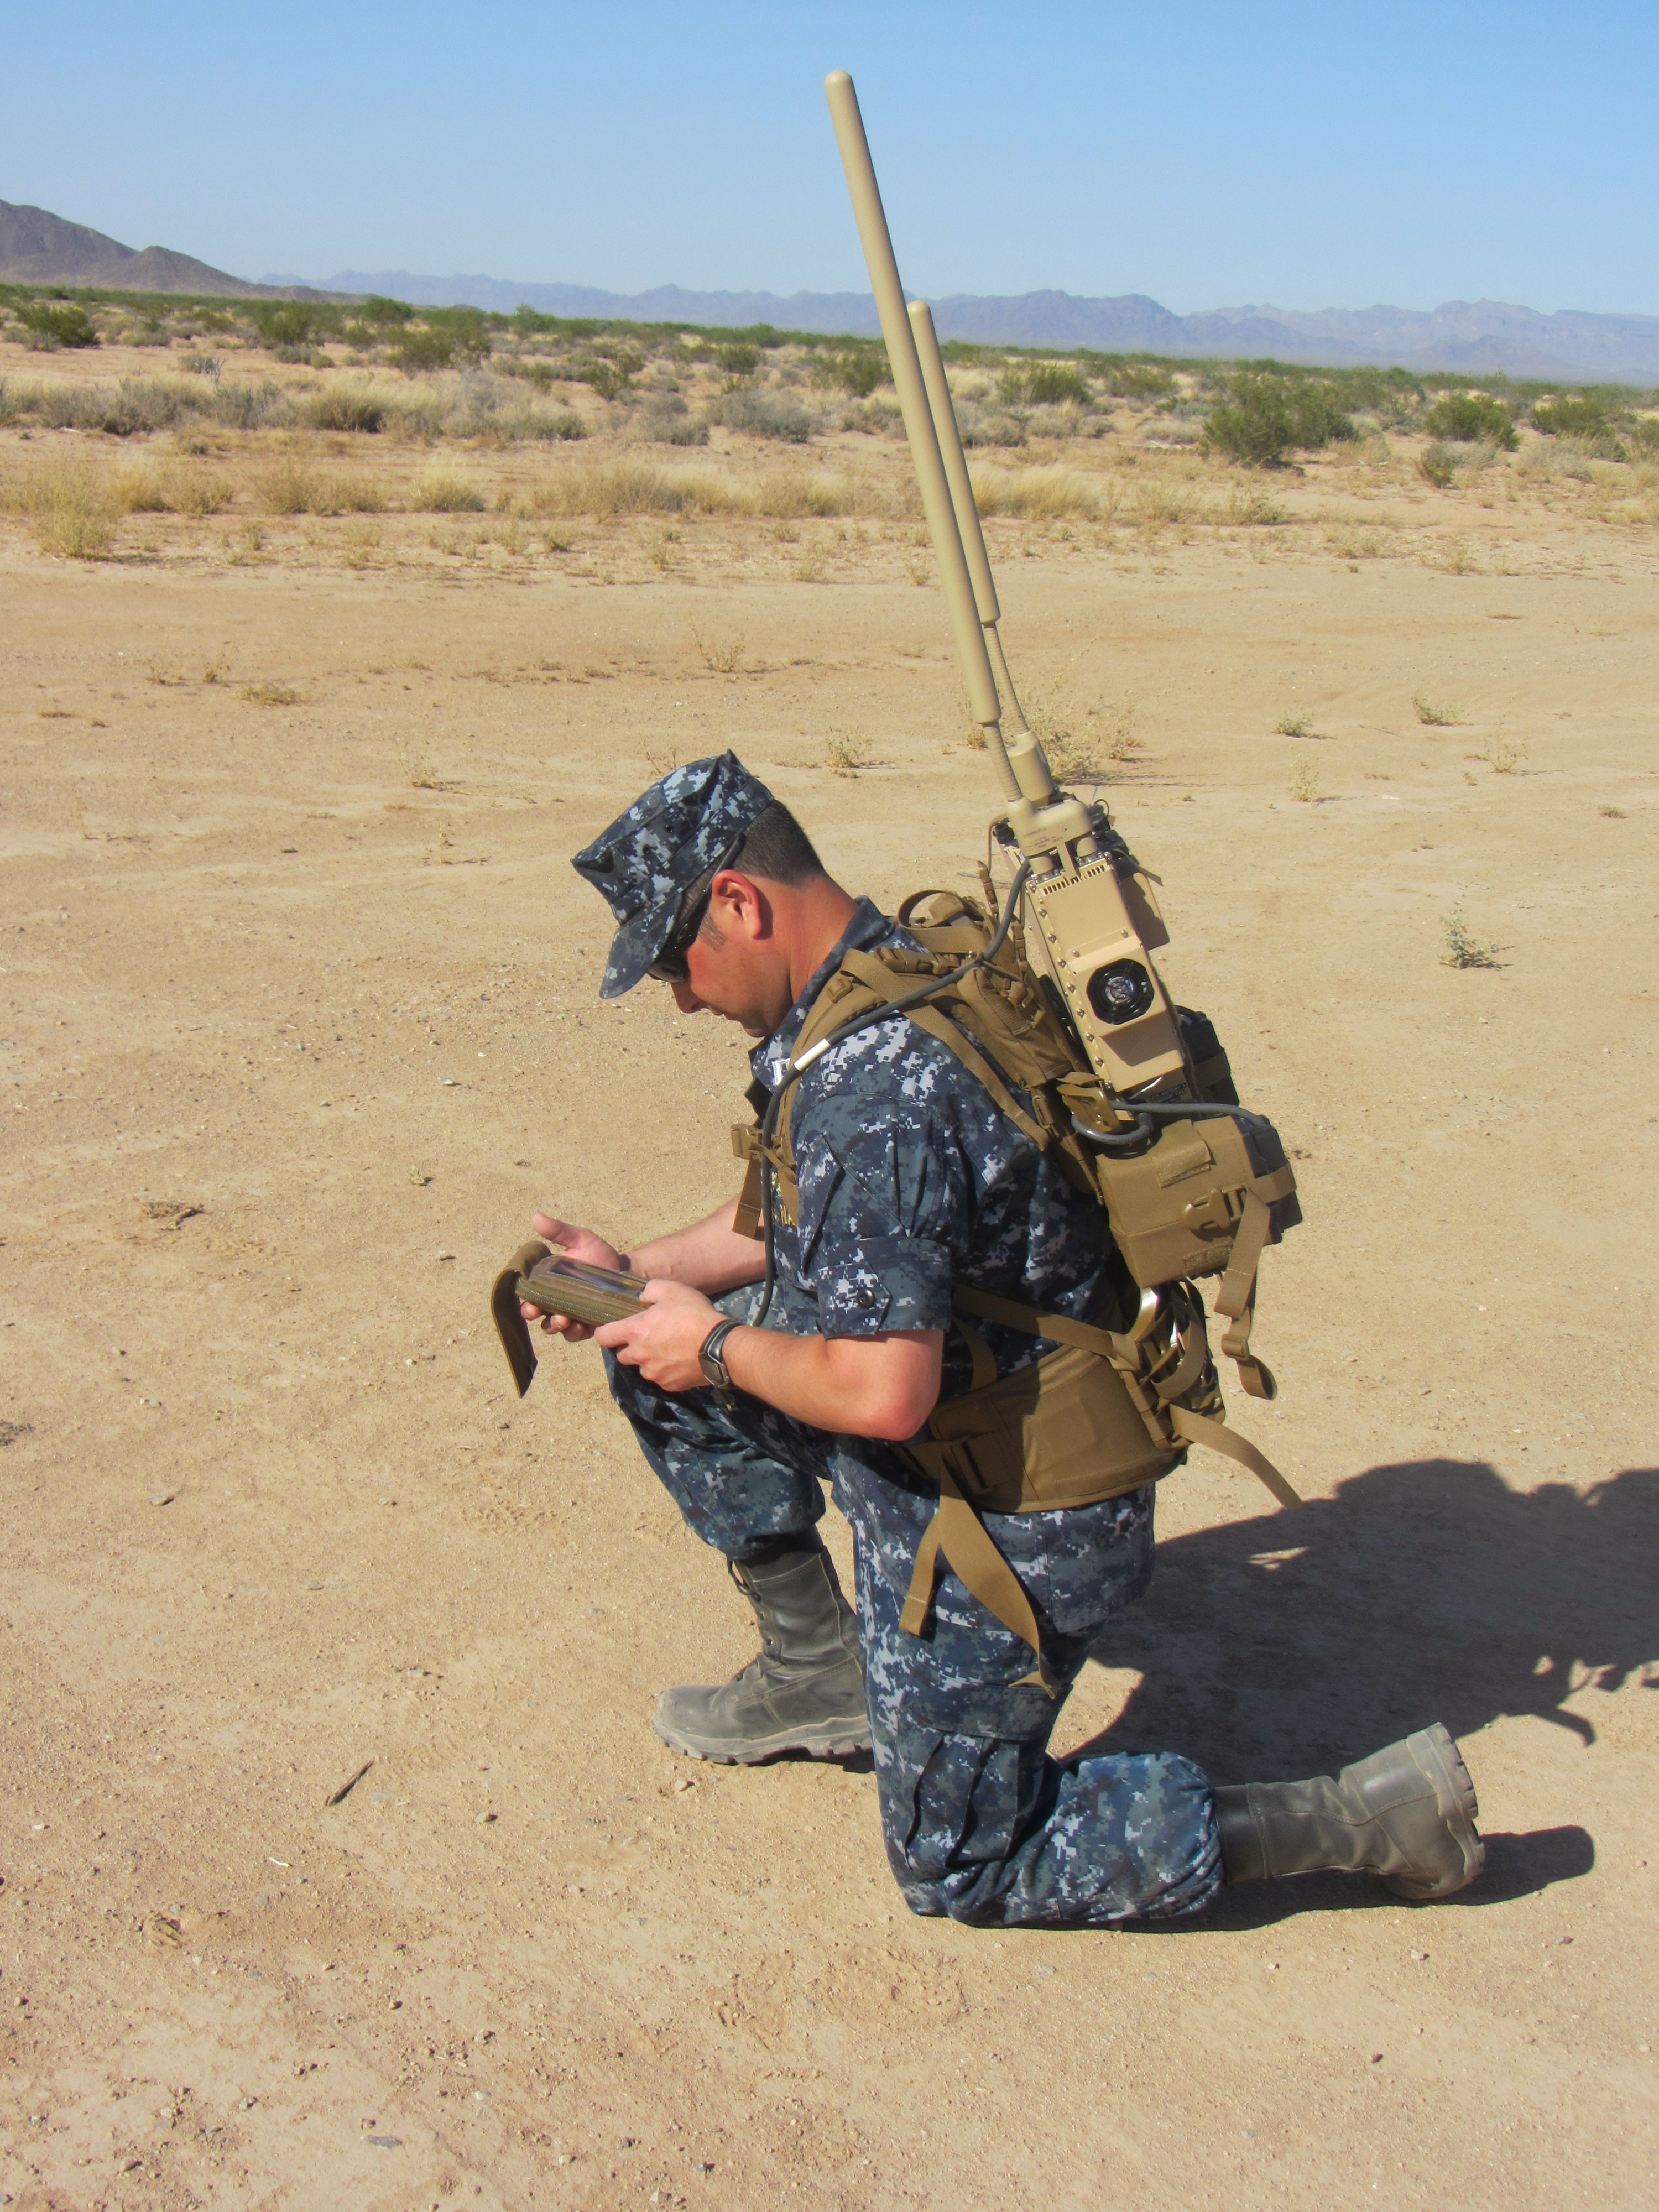
\includegraphics[width=\textwidth]{img/IED-jammers.jpg}
                % \caption{IED Jammers}
            \end{figure}

        \end{column}

    \end{columns}

\end{frame}



\begin{frame}{SAASM (Selective Availability Anti-Spoofing Module)}

    \begin{columns}[c, onlytextwidth]

        \begin{column}{0.35\textwidth}

            \begin{figure}
                \centering
                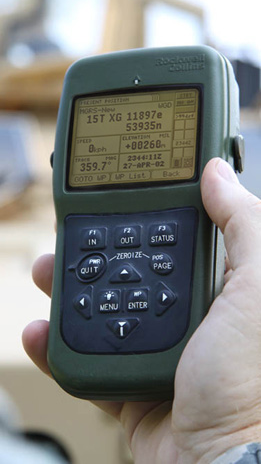
\includegraphics[width=\textwidth]{img/SAASM.png}
                % \caption{IED Jammers}
            \end{figure}

        \end{column}

        \hfill

        \begin{column}{0.6\textwidth}

            SAASM is a module that provides decryption and encryption capabilities to GPS receivers.

            \vspace{10pt}

            The use of a CSAC reduce the time needed to acquire the signal and allows the \textbf{use of longer GPS codes (encrypted P(Y) code)} that are less susceptible to jamming and spoofing.

        \end{column}

    \end{columns}

\end{frame}